\documentclass[tikz, border=1cm]{standalone}

\usepackage{tikz}
\usetikzlibrary{calc}

\begin{document}
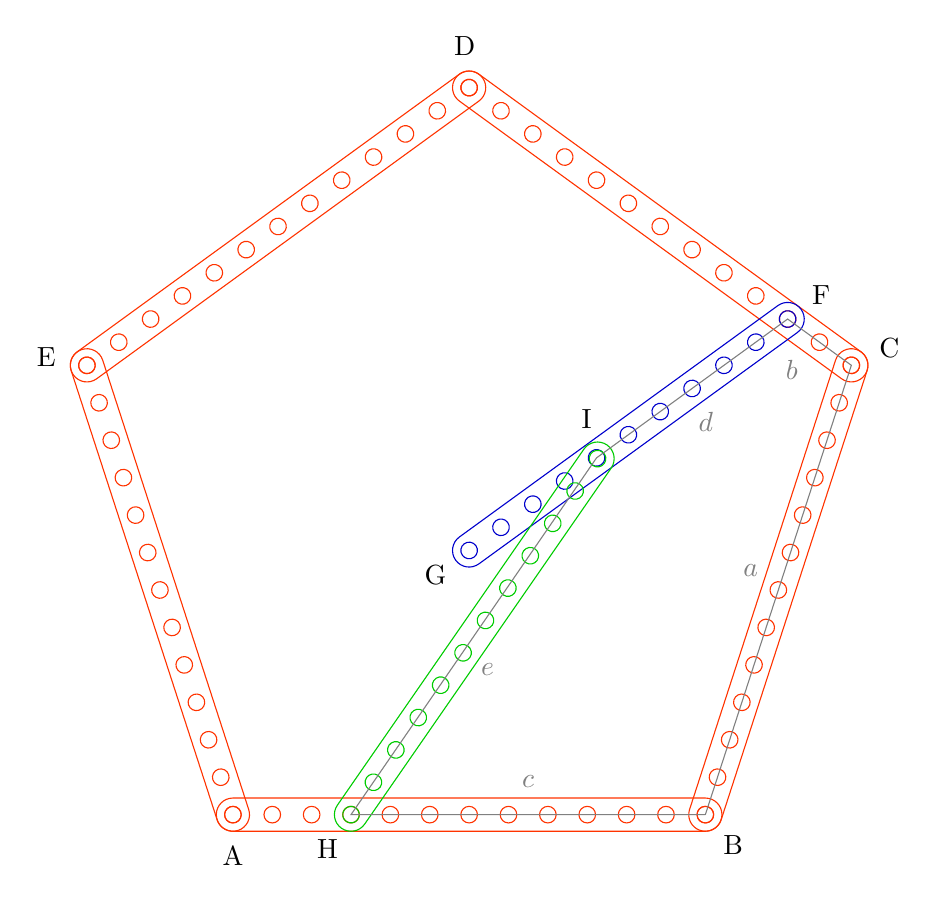
\begin{tikzpicture}

\newcommand{\rod}[4][000000] % [color][n][sep][prop]
{
 \definecolor{main}{HTML}{#1}
 \draw[main] (0,{{2*#4}})
   -- ++({#2*#3},0) arc(+90:-90:{2*#4})
   -- ++({-#2*#3},0) arc(270:90:{2*#4});
 \foreach \x in {0,1,...,#2}
  \draw[main] (\x*#3,0) circle (#4);
}

\newcommand{\pentagon}[5]
{
 \pgfmathsetmacro{\cosA}{cos(72)}
 \pgfmathsetmacro{\sinA}{sin(72)}
 \pgfmathsetmacro{\cosB}{cos(36)}
 \pgfmathsetmacro{\sinB}{sin(36)}

 \def\a{#1} 
 \def\b{#2}
 \def\c{#3}
 \def\d{#4}
 \def\e{#5}
 \def\f{0.5}\def\p {3pt}

 \def\red{FF3300} \def\blue{0000cc} \def\green{00cc00}
 \begin{scope}
  \rod[\red]{\a}{\f}{\p} \path (0,0) ++(270:5*\p) node{A};
  \begin{scope}[shift={(\a*\f,0)},rotate=72]
   \rod[\red]{\a}{\f}{\p} \path (0,0) ++(240:5*\p) node{B};
   \begin{scope}[shift={(\a*\f,0)},rotate=72]
    \rod[\red]{\a}{\f}{\p} \path (0,0) ++(240:5*\p) node{C};
    \begin{scope}[shift={(\a*\f,0)},rotate=72]
     \rod[\red]{\a}{\f}{\p} \path (0,0) ++(240:5*\p) node{D};
     \begin{scope}[shift={(\a*\f,0)},rotate=72]
       \rod[\red]{\a}{\f}{\p} \path (0,0) ++(240:5*\p) node{E};
     \end{scope}
    \end{scope}
   \end{scope}
  \end{scope}
 \end{scope}


 \def\Fx{\a*\f + \a*\f*\cosA - \b*\f*\cosB}
 \def\Fy{\a*\f*\sinA + \b*\f*\sinB}
 \begin{scope}[shift={(\Fx,\Fy)},rotate=180+36]
  \pgfmathsetmacro{\ab}{\a-\b}
  \rod[\blue]{\ab}{\f}{\p}
  \path (0,0) ++(180:5*\p) node{F};
  \path (\ab*\f,0) ++(0:5*\p) node{G};
 \end{scope}

 \pgfmathsetmacro{\cosA}{cos(72)}
 \pgfmathsetmacro{\sinA}{sin(72)}
 \pgfmathsetmacro{\cosB}{cos(36)}
 \pgfmathsetmacro{\sinB}{sin(36)}
 \pgfmathsetmacro{\ac}{\a - \c}

 \def\Hx{\ac*\f}
 \begin{scope}[shift={(\Hx,0)},rotate=55.3]
   \rod[\green]{\e}{\f}{\p}
   \path (0,0) ++(180:5*\p) node{H};
   \path (\e*\f,0) ++(50:5*\p) node{I};
 \end{scope}
 

 \coordinate (B) at (\a*\f,0);
 \coordinate (C) at (\a*\f + \a*\f*\cosA, \a*\f*\sinA);
 \coordinate (F) at (\a*\f + \a*\f*\cosA - \b*\f*\cosB, \a*\f*\sinA + \b*\f*\sinB);
 \coordinate (I) at (\a*\f + \a*\f*\cosA - \b*\f*\cosB - \d*\f*\cosB, \a*\f*\sinA + \b*\f*\sinB - \d*\f*\sinB);
 \coordinate (H) at (\ac*\f, 0);
 
 \draw[gray] (B)
 -- (C) node [midway,shift={(-1em,.7em)}]{$a$}
 -- (F) node [midway,shift={(-1em,-1em)}]{$b$}
 -- (I) node [midway,shift={(.5em,-1.2em)}]{$d$}
 -- (H) node [midway,shift={(.5em,-1.2em)}]{$e$}
 -- (B) node [midway,shift={(0,1.2em)}]{$c$}
 ; 
}

\pentagon{12}{2}{9}{6}{11}

\end{tikzpicture}
\end{document}
